\chapter{Gases of Moving Atoms}
In experiments, the motion and collisions of the atoms is another important factor that might impact the optical response of the gas. We have to face the possibility that the influence from the kinematics of the atoms could be so prominent that some cooperative effects may be more or less eliminated. It is worthwhile to extend our simulations to moving atoms. In fact, subsequent to the simulations of inhomogeneously broadened stationary atomic samples, we develop a code to deal with the atomic motion and the associated time evolution of the dipole moments. 

Inhomogeneous broadening is included in the simulations of moving atoms as it is a natural consequence of the thermal velocity distribution of the atoms. In the stationary-atom model, given a certain spatial distribution of the atoms, we are able to solve a closed set of linear equations to obtain the dipole moment of each atom.  However, in the moving-atom model, we integrate the equation of motion of each atom's dipole moment until  the gas reaches a steady state, and beyond. During that time, atoms undergo free flight as well as elastic collisions with the container walls and other atoms. Accordingly, we find that some kinematic factors such as the frequency of collisions may affect the simulation outcomes.

As expected, some results of stationary-atom simulations are inherited by moving-atom simulations, such as a dependence of collective Lamb shift on the sample thickness. Beyond that, some new features that do not exist in stationary-atom model  emerge. For instance, a typical Dicke narrowed lineshape~\cite{PhysRev.89.472} is observed.

However, contrary to what one might expect, as the gas density increases, the width of the Dick-narrowed central peak increases. This is quite unlike what would happen in a hypothetical gas of independent atoms, where, if anything, a higher density should lead to a reduced Dicke-narrowed linewidth. We attribute this broadening to the strong dipole-dipole interactions between the atoms, or from an overall perspective, to cooperative response of the gas to light. 

The following discussion is organized similarly as the preceding chapter on stationary atoms. We start from the analysis of one single moving atom, extend to many independent atoms, and finally focus on atoms with dipole-dipole interactions. Of course, the calculations and simulations are again done for a circular slab.

\section{Analysis of a one-atom gas}
In our model of discrete dipolar radiators, Eq.~\eq{CORE} can be specified so that it describes the time evolution of each atom's dipole moment. For the $n$th atom located at $\mathbf{r}_n$, we have
\bea
\dot{\mathbf{d}}(\mathbf{r}_n)&=&(i\Delta-\gamma)\mathbf{d}(\mathbf{r}_n)+i\zeta\mathbf{\mathcal{E}}_0(\mathbf{r}_n)+i\zeta\sum_{m\neq n}\mathsf{G}(\mathbf{r}_n-\mathbf{r}_m)\mathbf{d}(\mathbf{r}_m).
\label{DIPOLEEQ}
\eea
As before, $\Delta=\omega-\omega_0$ is the detuning from the atomic resonance $\omega_0$, $\gamma$ is the HWHM line width of the transition, $\zeta=\mathcal{D}^2/\hbar$ and $\mathcal{D}$ is the dipole matrix element, and $\mathbf{\mathcal{E}}_0$ is the electric field of the driving light if the matter were absent. $\mathsf{G}(\mathbf{r}_n-\mathbf{r}_m)$ is the dipole field propagator from the atom at $\mathbf{r}_m$ to the atom at $\mathbf{r}_n$. Atomic motion is taken into account in that the coordinates $\mathbf{r}_n$ change with time as the atoms move.

The first term on the right hand side of Eq.~\eq{DIPOLEEQ} comes from the damped free evolution of the atomic dipole. The second and the third terms, respectively, correspond to the dipole moment induced by the incident light and by the light scattered  from all other atoms. Evidently, if the left-hand side of Eq.~\eq{DIPOLEEQ} equaled zero, this equation would give the steady state as in Eq.~\eq{STEADY}.

All the calculations and simulations we present below are done under these universal conditions:
First, the gas sample is inside a circular disk with thickness $h$ and radius $R$. For convenience, the disk is placed so that its axis is used as the $z$ axis, and the body center is the coordinate origin. Unless explicitly stated otherwise, the area and radius of the disk are $A=256$ and $R=\sqrt{256/\pi}$.
Second, the incident light is represented by $\mathcal{E}_0(\mathbf{r})=E_0\,\hat{\mathbf{e}}\,e^{i\mathbf{k}\cdot\mathbf{r}}$. It is circularly polarized and propagates in the $+z$ direction,
\bea
\hat{\mathbf{e}}=-\{\frac{1}{\sqrt{2}},\frac{i}{\sqrt{2}},0\}, \, \mathbf{k}=\{0,0,1\}.
\eea
Third, the absorption spectrum is again investigated by calculating the optical thickness $D$ of the atomic sample as explained in Ref~\cite{0953-4075-44-19-195006}. 
Fourth, as some of the analytical expressions start swelling in size, we again resort to special units such that
\bea
k=c=\hbar=\frac{1}{4\pi\epsilon_0}=1;\quad \mathcal{D}=\sqrt{\frac{3\gamma}{2}}.
\label{UNITCONVENTION}
\eea 
These are also the units that are universally used in the numerical work.

\subsection{Dipole evolution of one atom}
\label{ONEATOMDIPOLE}
If the gas consists of only one atom, Eq.~\eq{DIPOLEEQ} can be reduced to an extraordinarily simple-looking inhomogeneous first-order ODE. Even if~\eq{UNITCONVENTION} already sets the units for all physical quantities, we introduce the added scaling of the running time that it is expressed in units of $\gamma^{-1}$, and find
\bea
\dot{\mathbf{d}}(t)+(1-i\delta)\mathbf{d}(t)=i\frac{3}{2}\mathcal{E}_0(t)=i\frac{3}{2}E_0\,\hat{\mathbf{e}}\,e^{i\mathbf{k}\cdot\mathbf{r}(t)}.
\label{SINGLEEQ}
\eea
Once more we define $\delta=\Delta/\gamma$. 

For $\mathbf{k}=\{0,0,1\}$, we readily have $\mathbf{k}\cdot\mathbf{r}(t)=z(t)=z_0+v_zt$. Thus, the radial components of the initial position and velocity have no effect on the evolution of the dipole. Likewise, we need not concern ourselves with elastic collisions between the atom and the lateral surfaces of the disk. As we will see in a moment, even the initial position $z_0$ eventually does not matter. Therefore, we endow the atom with the initial position $\mathbf{r}_0=\{0,0,-h/2\}$ and velocity $\mathbf{v}_0=\{0,0,v\}$ to carry out our analysis. This atom is sufficient to represent all the atoms that have the same axial speed $v$. For the time being, $v$ must be positive; because the atom is initially at $z=-h/2$, it has to move in the $+z$ direction to stay inside the disk.

We may take, for instance, 
\beq
\mathbf{d}_0=-\frac{3}{2(i+\delta)}E_0e^{-i\frac{h}{2}}\hat{\mathbf{e}}
\eeq
 as the initial dipole moment for the evolution, although the steady state that the dipole reaches after a long time is independent of the initial state as well. Anyway, given ${\bf d}_0$, the solution to Eq.~\eq{SINGLEEQ} is
\bea
d(t)&=&-\frac{3E_0}{2(i+\delta-v)}e^{i(-h/2+vt)}\left[1-e^{-t+i(\delta-v)t}\right]+e^{-t+i\delta t}d_0\,.
\label{SINGLESOL}
\eea
Note that we do not use the bold font anymore because the dipole moment always has the same polarization as the incoming electric field. The polarization $\hat{\mathbf{e}}$ can then be eliminated from the equation and everything is  scalar.

Obviously, the first term in Eq.~\eq{SINGLESOL} depends on the velocity on and the instantaneous electric field at the ever-changing position of the atom. The second term conveys the damping of the initial dipole. In free space, as time tends to infinity, the dipole moment would asymptotically approach
\bea
d(t\to\infty)=\alpha(v)E_0e^{i(-h/2+vt)},
\eea
where
\beq
\alpha(v)=-\frac{3}{2(i+\delta-v)}
\eeq
 is the Doppler-shifted polarizability of the atom with the speed $v$.

However, the atom is confined to the disk. In our model it experiences elastic collisions with the end caps of the disk at $z=\pm h/2$, whereupon the direction of the velocity reverses. The time interval between any two successive collisions  is $h/v$. At the time $h/v$ the first collision happens at $z=h/2$, and the dipole is
\bea
d_1\equiv d(t=\frac{h}{v})&=&\alpha(v)E_0 e^{ih/2}\left[1-e^{-\frac{h}{v}+i(\delta-v)\frac{h}{v}}\right]+e^{-\frac{h}{v}+i\delta \frac{h}{v}}d_0.
\eea
$d_1$ would in turn serve as the initial state to obtain the dipole at the second collision, $d_2$. Note that this time $v$ is replaced by $-v$ as the atom bounces back after the first collision:
\bea
d_2&=&\alpha(-v)E_0e^{-ih/2}\left[1-e^{-\frac{h}{v}+i(\delta+v)\frac{h}{v}}\right]+e^{-\frac{h}{v}+i\delta \frac{h}{v}}d_1\nonumber\\
&=&\alpha(-v)E_0e^{-ih/2}\left[1-e^{-\frac{h}{v}+i(\delta+v)\frac{h}{v}}\right]+\alpha(v)E_0e^{ih/2}\left[1-e^{-\frac{h}{v}+i(\delta-v)\frac{h}{v}}\right]e^{-\frac{h}{v}+i\delta \frac{h}{v}}\nonumber\\
&&+(e^{-\frac{h}{v}+i\delta \frac{h}{v}})^2d_0\nonumber\\
&=&d_+q+d_-+q^2d_0.
\eea
Here we have defined
\bea
d_+&=&\alpha(v)E_0e^{ih/2}\left[1-e^{-\frac{h}{v}+i(\delta-v)\frac{h}{v}}\right],\nonumber\\
d_-&=&\alpha(-v)E_0e^{-ih/2}\left[1-e^{-\frac{h}{v}+i(\delta+v)\frac{h}{v}}\right], \nonumber\\
q&=&e^{-\frac{h}{v}+i\delta \frac{h}{v}}
\eea
for a more compact notation.

Now we can inductively write out the dipole moment at the $n$th collision as 

\begin{subequations}
\begin{numcases}{d_n=}
d_+\sum_{k=0}^{\frac{n-1}{2}}q^{2k}+d_-\sum_{k=0}^{\frac{n-3}{2}}q^{2k+1}+q^nd_0, &($n$ is odd and $n\geq 3$) \\
 \nonumber\\
d_+ \sum_{k=0}^{\frac{n-2}{2}}q^{2k+1}+d_- \sum_{k=0}^{\frac{n-2}{2}}q^{2k}+q^nd_0. &($n$ is even and $n\geq 2$)
\end{numcases}
\end{subequations}
Since $\left|q\right|<1$, the summations converge as $n\to\infty$ so that we have
\begin{subequations}
\begin{numcases}{d_{n\to\infty}=}
\frac{d_++qd_-}{1-q^2} \,, & \textrm{(odd $n$)}\label{FINAL1}\\
\nonumber\\
\frac{qd_++d_-}{1-q^2}\,. & \textrm{(even $n$)}.\label{FINAL2}
\end{numcases}
\end{subequations}
If we wait long enough, the time evolution eventually leads to an alternation of the dipole moment between the values~\eq{FINAL1} and~\eq{FINAL2} when the atom bounces off the endcaps. In steady state the dipole moment is equal to~\eq{FINAL1} when the atom arrives at the endcap at $z=h/2$ and equal to~\eq{FINAL2} when it is at $z=-h/2$.

Between the two ends of the cylinder, the dipole moment still evolves according to Eq.~\eq{SINGLESOL}. The oscillations of the dipole moment are synchronized with the kinematic oscillations. The period of both oscillations equals the duration of a round trip between the two endcaps, which is $2h/v$.

Consider the dipole moment over one period, starting the time when the atom is at $z=-h/2$. In the first half of the period the dipole moment is
\bea
d_{F}(t)&=&\alpha(v)E_0e^{ih/2}\left[1-e^{-t+i(\delta-v)t}\right]+q(qd_++d_-)\frac{1}{1-q^2}.
\label{FORWARD}
\eea
We zero the timer again when the atom reaches $z=h/2$, so that during the return trip the dipole is
\bea
d_{B}(t)&=&\alpha(-v)E_0e^{-ih/2}\left[1-e^{-t+i(\delta+v)t}\right]+q(d_++qd_-)\frac{1}{1-q^2}.
\label{BACKWARD}
\eea
Combining Eq.~\eq{FORWARD} and Eq.~\eq{BACKWARD}, we are able to write out the dipole moment at any time within one period,
\begin{numcases}{d(t)=}
d_F(t), & ($0\leq t\leq  h/v$)\nonumber\\
d_B(t-h/v). & ($h/v \leq t \leq 2h/v)$
\label{BACKFORTH}
\end{numcases}

\subsection{Optical thickness}
For the present purposes let us write the optical thickness as $D=-\ln|\tau|^2$,
where $\tau$ is the amplitude transmission coefficient. Now, compared with all other time scales of the problem, the propagation of the light across the disk is typically instantaneous. We may therefore define an instantaneous amplitude transmission coefficient, and optical thickness as well. We again use the forward-scattering approximation of Ref.~\cite{1367-2630-14-5-055001}, see Eq.~\eq{TRLIGHT} and also Ref.~\cite{0953-4075-44-19-195006}. The dipole moment is actually an explicit function of $h$, $v$, $\delta$ and $t$, so we write it as $d(h,v,\delta,t)$, and have the amplitude transmission coefficient for a single atom
\bea
\tau_1=1+\frac{2ie^{-iz(t)}d(h,v,\delta,t)}{R^2E_0},
\eea
where $z(t)$ is the position of the atom at time $t$. The phase of this transmission coefficient is referenced to $z=0$; multiply by $e^{ih/2}$ for the amplitude transmission coefficient at the exit face of the disk.

The optical thickness $D_1$ is
\bea
D_1(h,v,\delta,t)&=&\ln\left|\tau_1\right|^{-2}=-\ln\left|\tau_1\right|^2=-\ln(\tau_1\tau_1^*)\nonumber\\
&=&-\ln\Bigg\{1+2\,\mathfrak{R}\left[\frac{2ie^{-iz(t)}}{R^2}\frac{d(h,v,\delta,t)}{E_0}\right]\nonumber\\
&&+\left|\frac{2ie^{-iz(t)}}{R^2}\frac{d(h,v,\delta,t)}{E_0}\right|^2\Bigg\}.
\eea
For $R\gg1$, we have the approximation
\bea
D_1(h,\delta,v,t)&\approx&-\ln\left(1+2\,\mathfrak{R}\left[\frac{2ie^{-iz(t)}}{R^2}\frac{d(h,v,\delta,t)}{E_0}\right]\right)\nonumber\\
&\approx&-\frac{4}{R^2E_0}\mathfrak{R}\left[ie^{-iz(t)}d(h,v,\delta,t)\right].
\label{APPROX}
\eea

As we discussed in Sec.~\ref{ONEATOMDIPOLE}, $z(t)$ and $d(h,v,\delta,t)$ are oscillating in phase, so the time average of the optical thickness can be calculated by integrating the term in the square brackets over a round trip of the atom and dividing the result by the round-trip time $2h/v$,
 \bea
\bar{D}_1(h,v,\delta)&=&-\frac{4}{R^2E_0}\mathfrak{R}\left[\frac{v}{2h}\int_0^{\frac{2h}{v}} ie^{-iz(t)} d(h,v,\delta,t)dt\right]\nonumber\\
&=&\frac{4}{R^2}\mathfrak{R}\Bigg\{\frac{3v^3\left[{\rm coth}(\frac{h-ih\delta}{v})-\cos(h){\rm csch}(\frac{h-ih\delta}{v})\right]}{h(i+\delta-v)^2(i+\delta+v)^2}\nonumber\\
&&-\frac{3(1-i\delta)}{2(i+\delta-v)(i+\delta+v)}\Bigg\}.
\label{THEORYD}
\eea
As the final step, we imagine an ensemble of an infinite number of one-atom samples in which the atom's axial velocity obeys the Gaussian distribution with zero mean and rms axial velocity (standard deviation) equal to $u$. Then the ensemble-averaged absorption spectrum is
\bea
D_1(h,u,\delta)=\int_{-\infty}^{\infty}\bar{D}_1(h,v,\delta)\frac{e^{-\frac{v^2}{2u^2}}}{\sqrt{2\pi}\,u}dv.
\label{ONEATOMSPECTRUM}
\eea

We numerically compute and plot $D_1(\delta)$ versus $\delta$ in  Fig.~\ref{SINGLESPECTRUM} for certain values of $h$ and $u$. The lines are from~Eq.~\eq{ONEATOMSPECTRUM}. The markers give outcomes from the corresponding direct numerical simulations, to be explained in detail below.
\begin{figure}[h!]
\begin{center}
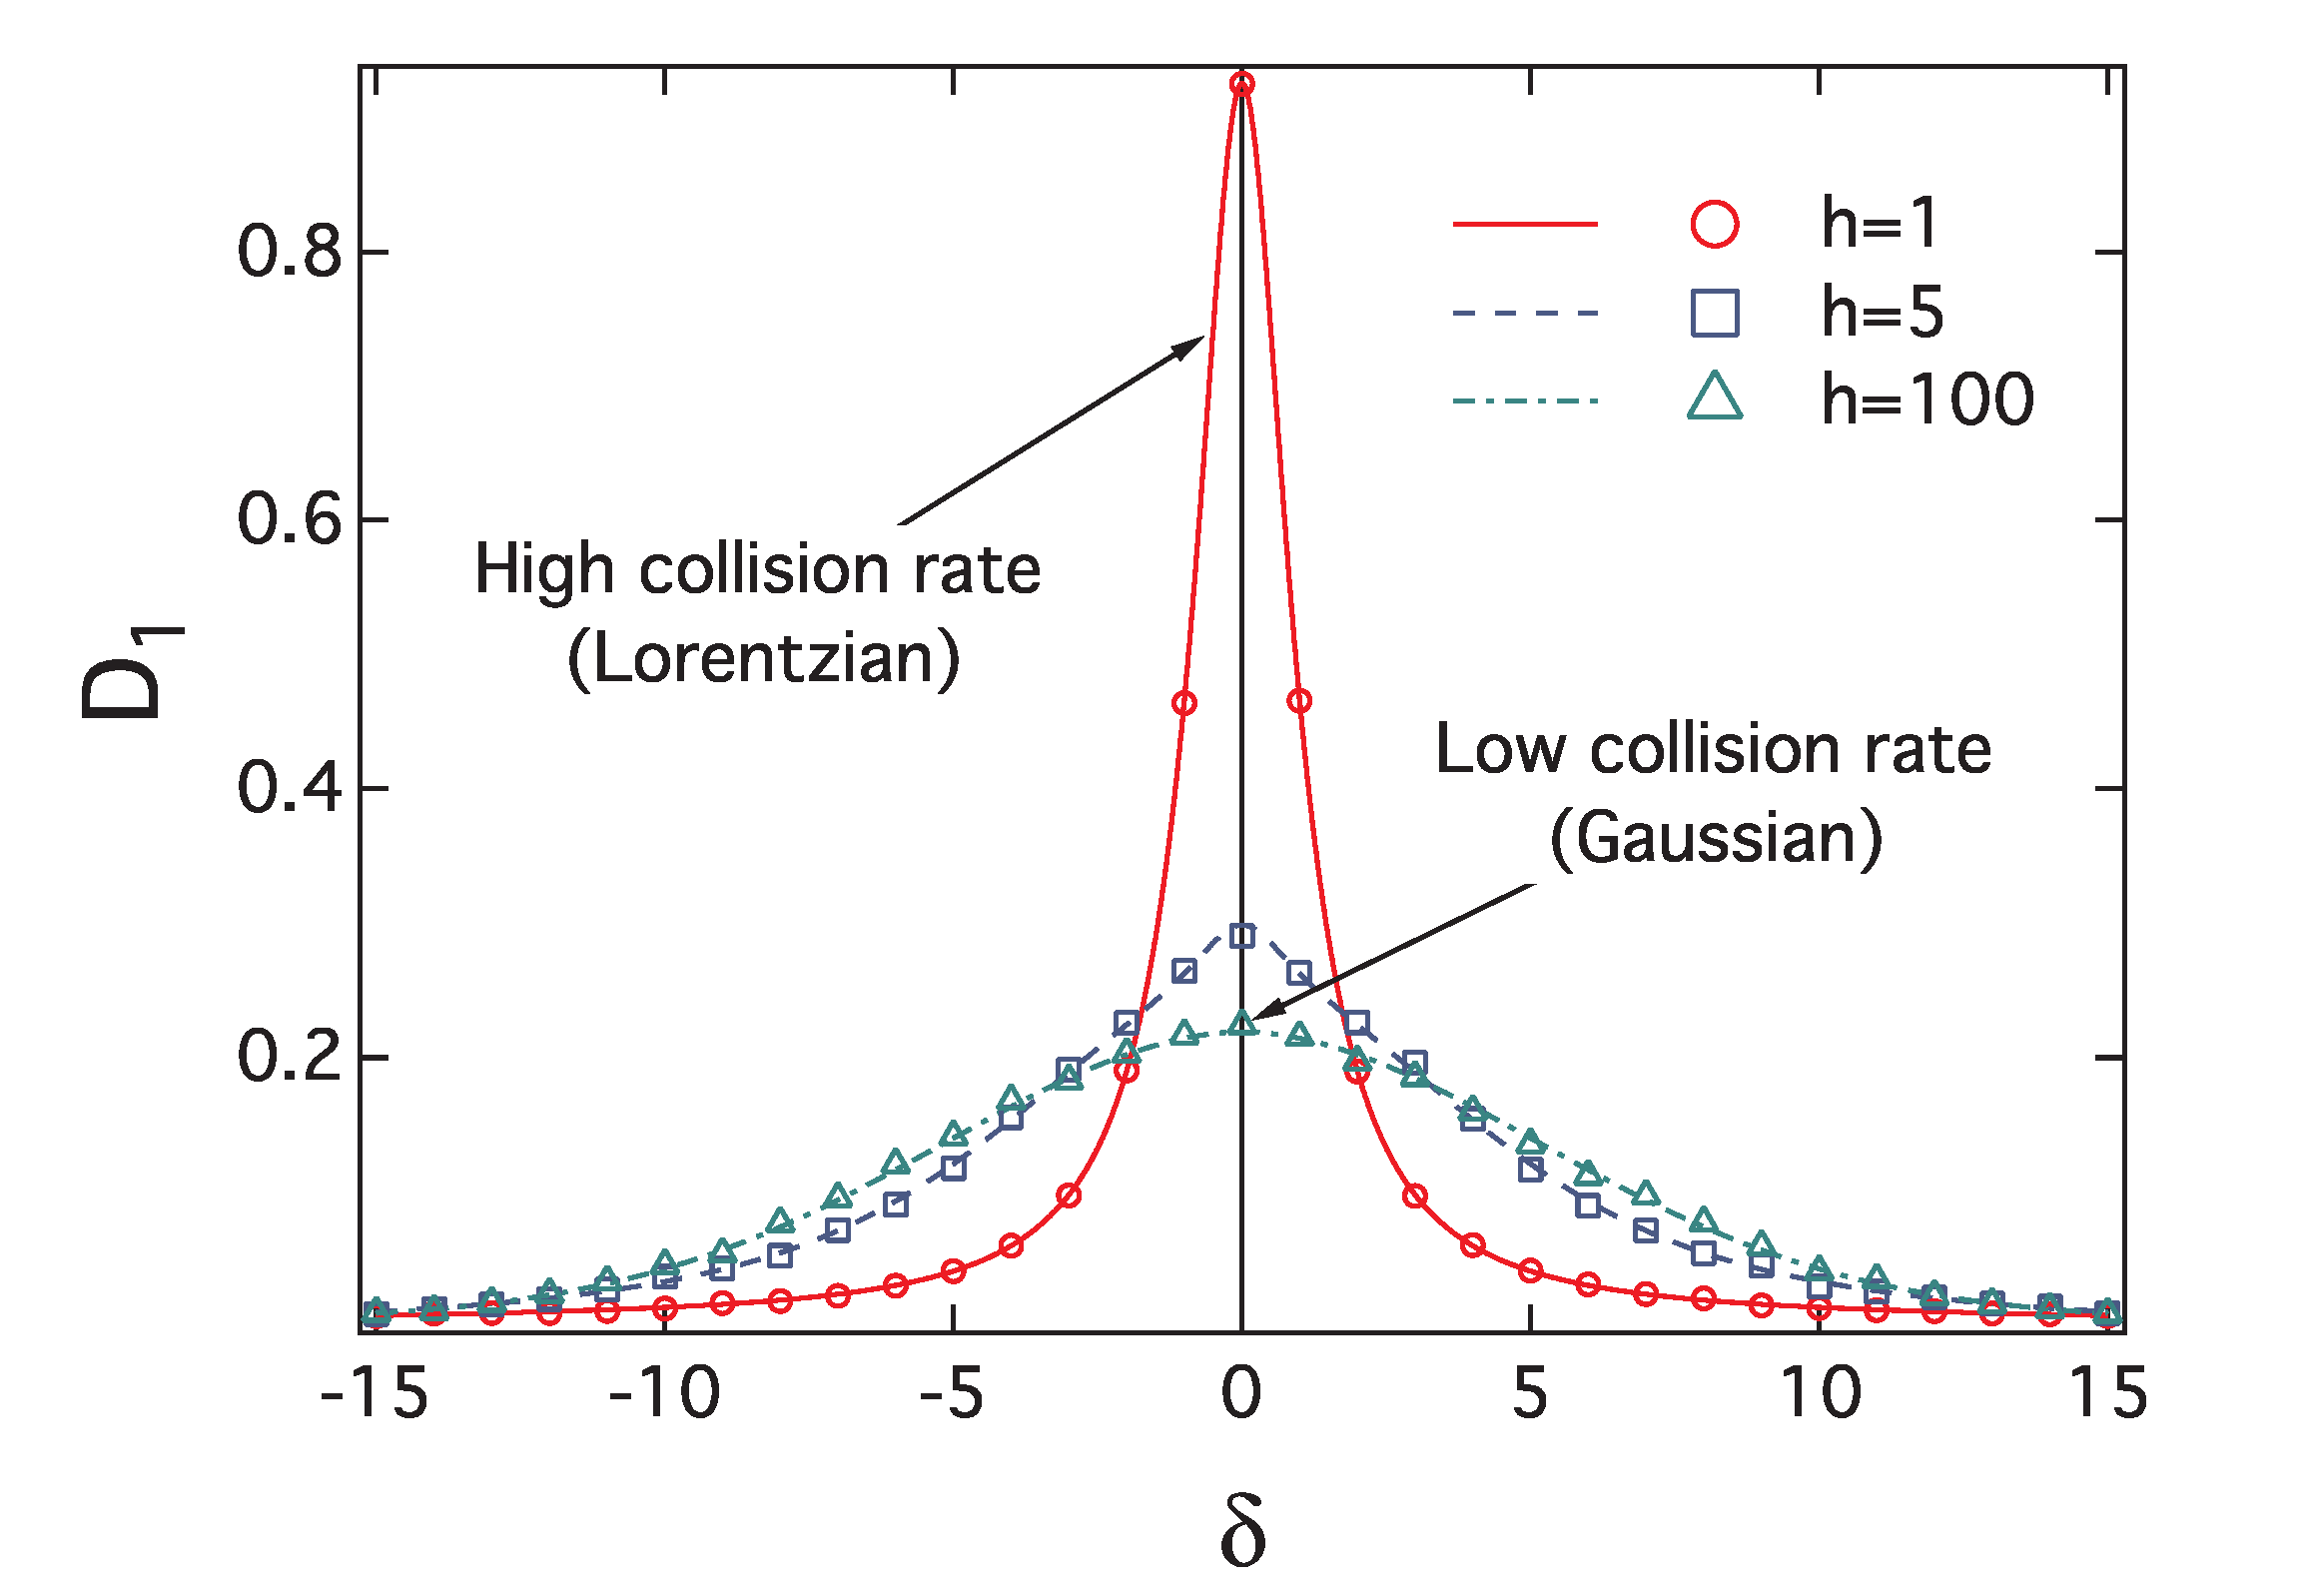
\includegraphics[width=\textwidth]{single_atom.pdf}
\end{center}
\caption{Optical thickness $D_1$ versus detuning $\delta$ of a single-atom ensemble with disk thicknesses $h=100, 5$ and $1$. The rms axial speed of the atom is $v=5$ for all of the data. Continuous lines are results from Eq.~\eq{ONEATOMSPECTRUM}, discrete markers give results from the corresponding direct numerical simulations. Essentially Gaussian and Lorentzian profiles are observed for $h=100$ and $h=1$, respectively. When $h=5$, a bulge close to resonance makes the lineshape intermediate between a Gaussian and a Lorentzian. Numerical simulations agree with the analytical calculations.}
\label{SINGLESPECTRUM}
\end{figure}

The three curves in  Fig.~\ref{SINGLESPECTRUM} reveal an important phenomenon. As we keep the rms speed of the atom constant and vary the thickness $h$ from very large to very small, the spectrum undergoes a transition from a broad Gaussian line to a narrow Lorentzian. This transition is consistent with Dicke narrowing~\cite{PhysRev.89.472}. Basically, if an atom were to fly freely in space, a situation approximated at the thickness $h=100$, the motion adds a Doppler shift to the atomic resonance frequency that can be detected spectroscopically. On the other hand, if collisions confine the atom to a region small compared to the wavelength of light, as in the case $h=1$, then the atom-field interaction is as if the atom were stationary. The case $h=5$ is intermediate between the two extreme cases, and shows an intermediate spectrum. 

\subsection{A simplified many-atom gas}
\label{SMAG}

We can make one more step forward with a simplified model of a gas of $N$ atoms.
So far the atom radius is taken to be infinitesimal, hence there are no atom-atom collisions. Moreover, the dipole-dipole interaction between the atoms is neglected, hence there are neither collisions as a result of the forces between the dipoles, nor cooperative radiative properties. Under these conditions each atom evolves independently of the others, and the dipole moment of each atom in steady state is still given by Eq.~\eq{BACKFORTH}. 

If we have $\{v_n\}$ $(n=1,2,3,\cdots,N)$ as the speeds of the $N$ atoms, the total amplitude transmission coefficient can be written
\bea
\tau_N=1+\sum_{n=1}^{N}\frac{2ie^{-iz_n(t)}d(h,\delta,v_n,t)}{R^2E_0},
\eea
where $z_n(t)$ is the ever-changing position of the $n$th atom. 

Like before, we assume $R\gg 1$, so the approximation in Eq.~\eq{APPROX} is still valid and the total optical thickness of the gas is
\bea
D_N(h,\{v_n\}, \delta,t)&\approx&-\frac{4}{R^2E_0}\mathfrak{R}\left[\sum_{n=1}^{N}ie^{-iz_n(t)}d(h,\delta,v_n,t)\right]=\sum_{n=1}^{N}D_1(h,v_n,\delta,t).\nonumber\\
\eea
Note that the sum and the time integral in Eq.~\eq{THEORYD} are interchangeable, so the time average is
\bea
\bar{D}_N(h,\{v_n\},\delta)=\sum_{n=1}^{N}\bar{D}_1(h,v_n,\delta).
\eea
Finally, if all of the $v_n$ have a Gaussian distribution with the rms velocity $u$, the absorption spectrum of the N-atom gas is
\bea
D_N(h,u,\delta)=ND_1(h,u,\delta).
\eea

We can see that, except for a multiplying factor $N$, the spectrum from such a simplified model of a gas is identical to the spectrum of a single atom, as in Fig.~\ref{SINGLESPECTRUM}. 
 
This is as far as we can get analytically, up to quadrature. As we want to investigate the influence of atom-atom collisions on the spectrum next, we have to turn to simulations.

The details of our simulations will be explained in next section. Here, as a preview, we present simulation results for a gas of $N$ atoms with and without atom-atom collisions in Fig.~\ref{COLLISION}. However, dipole-dipole interactions are still not included in either analytical results or in numerical simulations. It is clear that, as we adopt a large atom radius so that atom-atom collisions become prevalent, the line shape significantly narrows.

\begin{figure}[h!]
\begin{center}
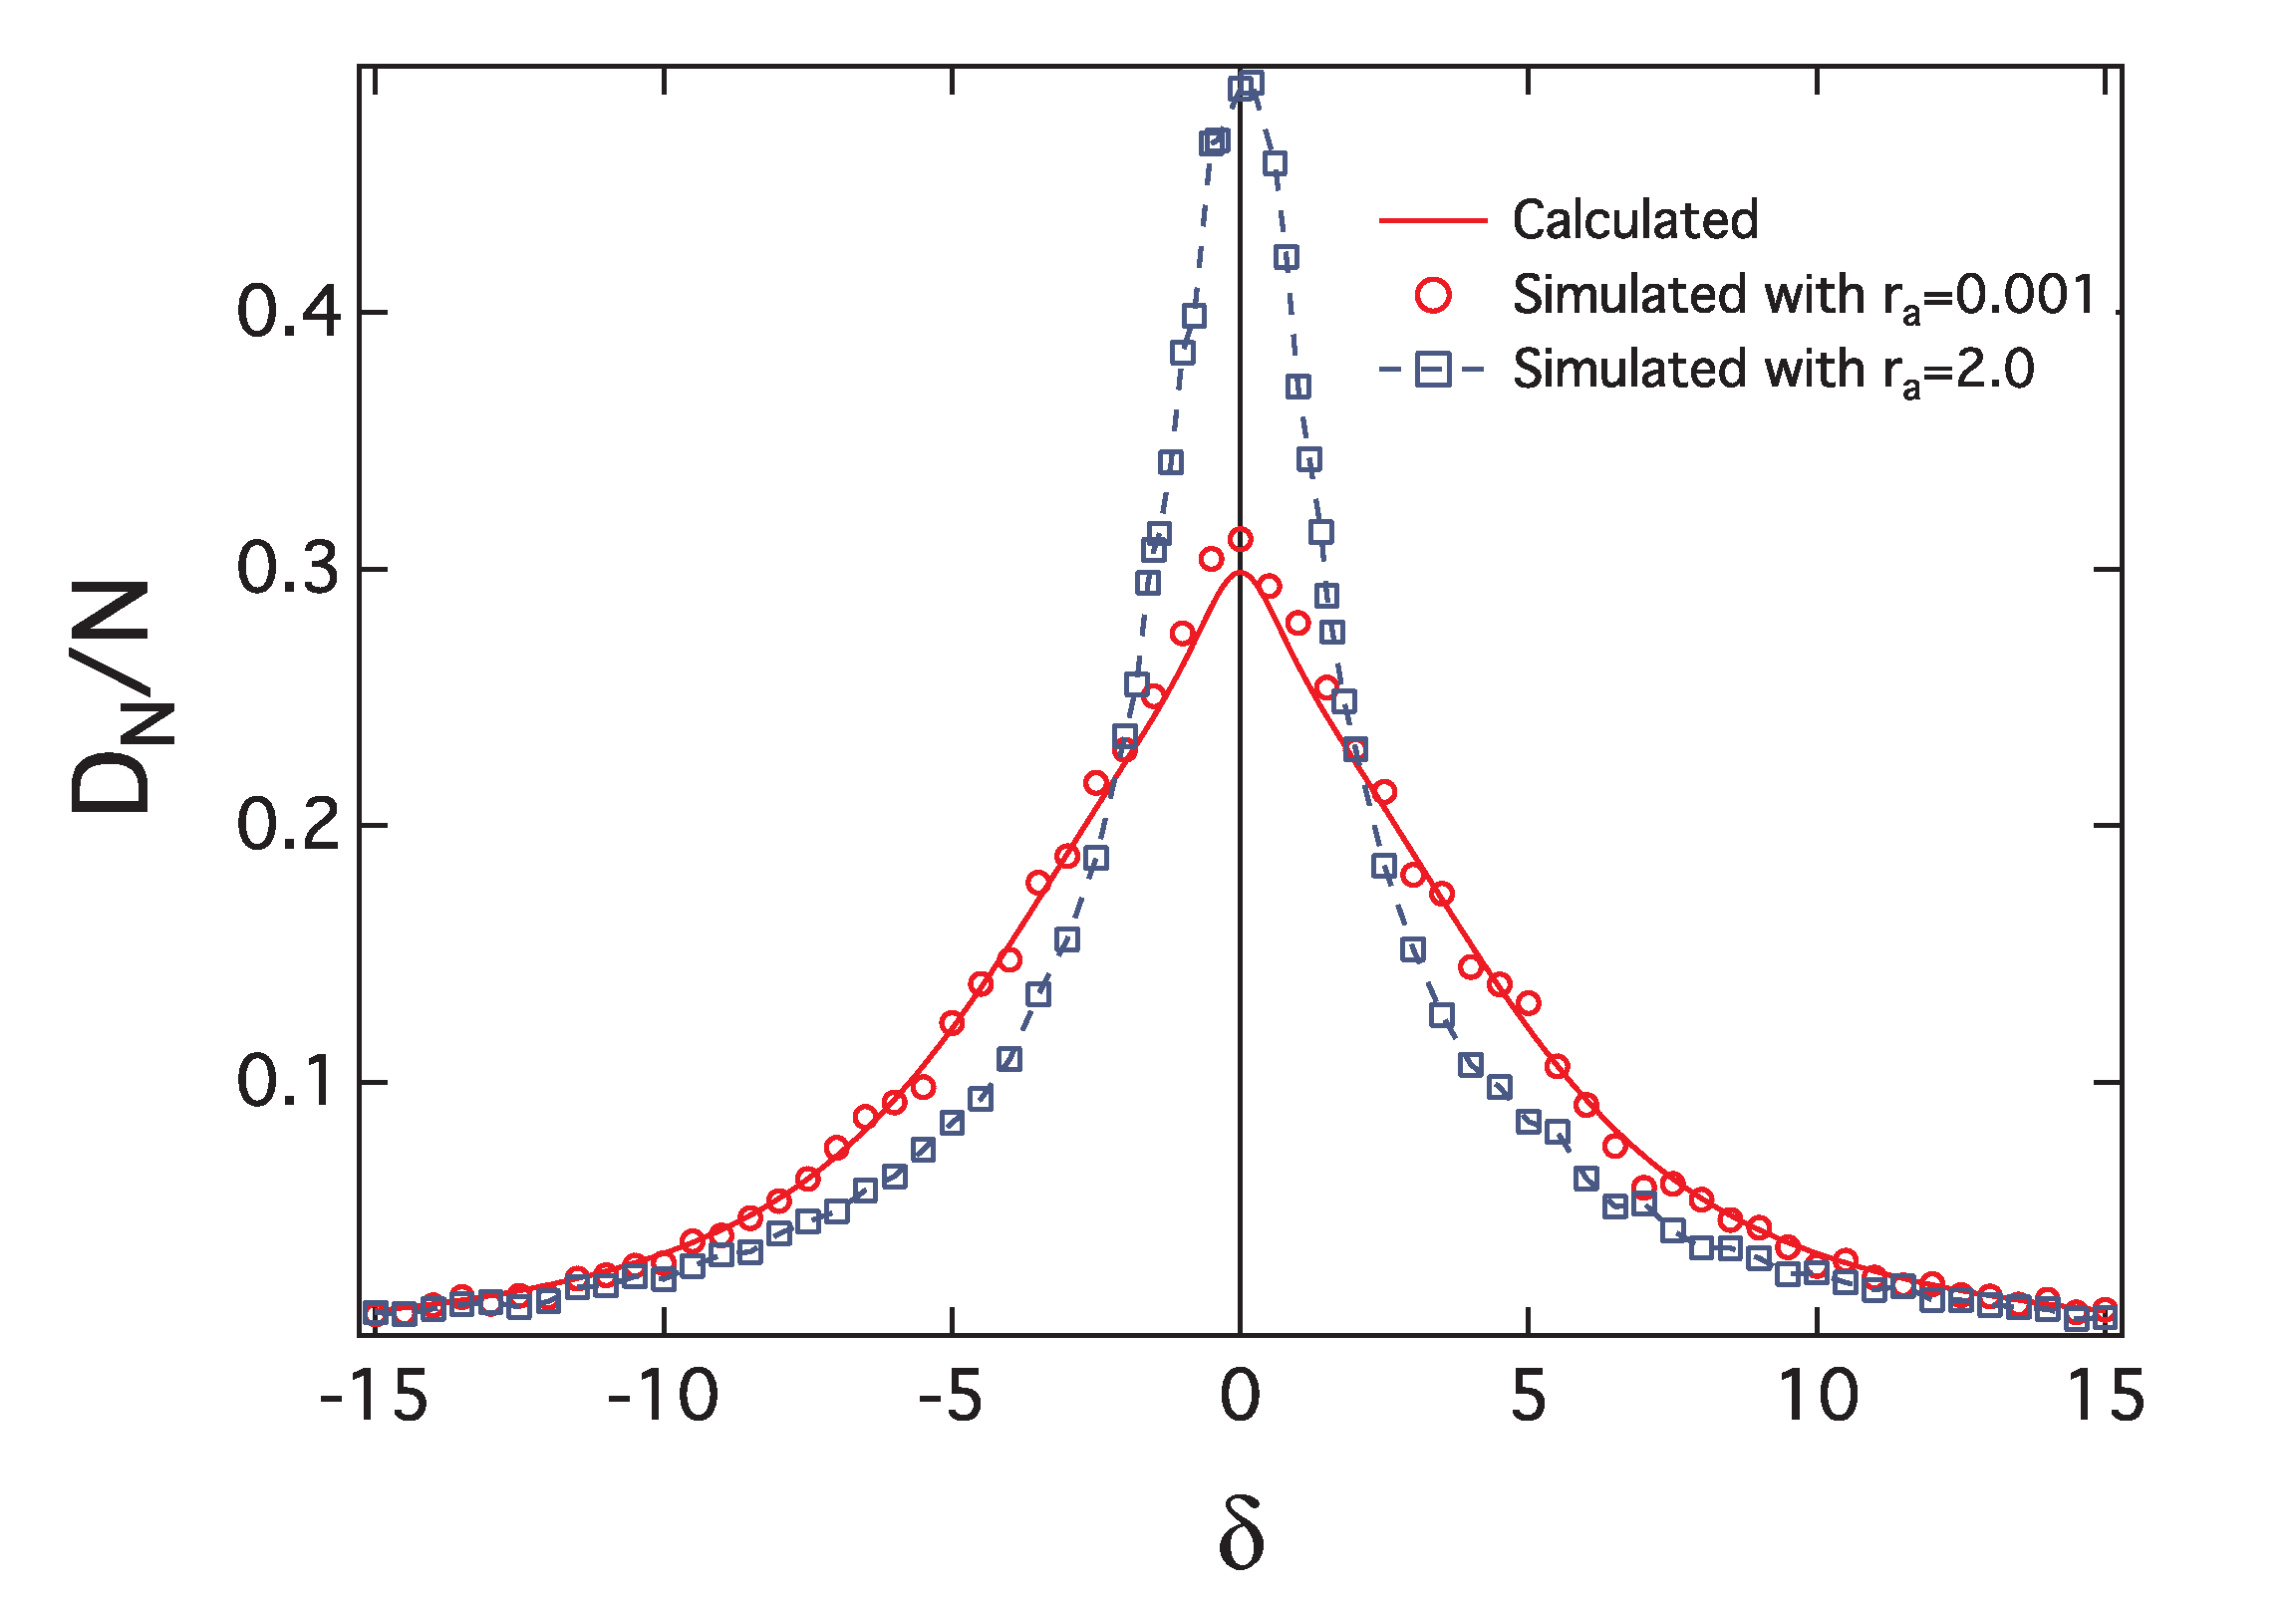
\includegraphics[width=\textwidth]{COLLISION.pdf}
\end{center}
\caption{Optical thickness per atom $D_N/N$ versus detuning from resonance $\delta$ with different atom-atom collision rates if there were no dipole-dipole interactions. The solid line is from Eq.~\eq{ONEATOMSPECTRUM}, and is identical to $D_1$ with $h=5$ in Fig.~\ref{SINGLESPECTRUM}. The red circles correspond to simulations where the atom radius was $r_a=0.001$, and the simulation programs recorded no atom-atom collisions at all. The blue boxes are for simulations with $r_a=2.0$, so about half of the collisions of the atoms are mutual collisions and half are collisions with the walls of the container. In all cases, $N=10$, $u=5$, $R=\sqrt{256/\pi}$ and $h=5$.}
\label{COLLISION}
\end{figure}
In summary, if the dipole-dipole interactions between the atoms were completely absent, either by shortening the disk in the $z$-direction or by increasing the atom radius we would end up with a narrowing lineshape in the absorption spectrum. The essential mechanism is the same in both cases: the mean free path of the atoms is reduced, and the resulting confinement leads to Dicke narrowing.

\section{Simulations of many-atom gases}
\subsection{Procedure and validity of the simulation program}

Most of our effort is put into simulations that include the dipole-dipole interactions. First of all, some details about the simulations will be discussed. 

\subsubsection{Initial state of the evolution}

We assume that, initially, the gas sample is evenly distributed inside the circular disk. The atoms obey the Maxwell-Boltzmann velocity distribution and have the same root-mean-square velocity in all three orthogonal directions.

Although the initial  dipole moments of the atoms are irrelevant to the eventual steady state, it is still worthwhile to  choose the initial state carefully so that the system relaxes to the steady state as quickly as possible. This is critical when we deal with a large number of atoms: The efficiency of the computations becomes a major concern, especially as this numerical problem is not a good match to the paradigm underlying Open Science Grid.

In our simulations, after the initializations of the positions and velocities, the first step is to solve the same equations for the dipole moments of the atoms as in a stationary-atom simulation with inhomogeneous broadening. The resonance frequency of each atom is simply Doppler-shifted by $\Delta\omega=kv_z$. The solutions to these $6N$ linear equations provide the initial state for the dipole evolution described by Eq.~\eq{DIPOLEEQ}.

\subsubsection{Integration of the evolution equations and sampling}

We use adaptive-stepsize Runge-Kutta method to integrate Eq.~\eq{DIPOLEEQ} numerically. The coordinates of the $n$th atom $\mathbf{r}_n$ change with time as the atom moves. Between two successive collisions, the displacement of all atoms is linear to time. However, this linear dependence is interrupted by collisions.

As to collisions, an atom is conceptually treated as hard sphere with the radius $r_a$. Each atom may collide either with another atom, or with the inside wall of the container. All collisions are assumed elastic. Again conceptually (implementations may differ on this), we artificially enlarge the stated radius and thickness of the disk, 
$R\rightarrow R+r_a$ and $h\rightarrow h+2r_a$, so that the center-of-mass of each atom has the entire volume $\pi R^2h$ available to it.

In more algorithmic detail, we use the data structures available in the Standard Template Library of C++ to maintain a record (a ``map'' in one particular implementation) of the next known collision for each atom; when and where will it happen, is it an atom-atom collision or a collision with a container wall. The atom that collides first obviously determines the next collision overall. At a collision both the atomic velocities and the record of the next known collision for each atom are updated appropriately. Between the collisions, the atoms simply fly ballistically. This algorithm has proven very efficient. In the cases when we have profiled the code, it has spent most of the time computing the dipole-dipole interactions.

When a collision happens,  we halt the Runge-Kutta integration, update the atom or atoms that just collided with the new velocity or velocities, and then resume the integration.

It may be noted that we have also studied the motion of the atoms with the collisions but without integrating the dipole moments. This is in order to test the system that manages the motion of the atoms. The results have been satisfactory. For instance, we have seen a monoenergetic distribution of atomic velocities relax to a Maxwell-Boltzmann velocity distribution as expected.

In the simulations with stationary atoms we take the average over many statistically independent static samples. Now we may also work with time averages in one sample.  We wait for a time much longer (say, ten times longer) than the relaxation time of the system to reach a steady state, and then begin to take snapshots of the quantity we wish to analyze. The time interval between the snapshots should also be longer than the relaxation time to ensure the statistical independence of the samples. Each snapshot works as a sample in our analysis. 

The caveat here is that the relaxation time has proven difficult to determine. One could, for instance, start the system from a state far from equilibrium and follow the optical thickness relax to a constant. Alternatively, on could analyze the fluctuations of the samples in the purported steady state as a function of the time interval between the samples to get an idea of how statistically independent the samples are. The unfortunate fact is that the results for the relaxation time from such different methods may easily differ by an order of magnitude.

\subsubsection{Collective Lamb shift for moving atoms}
 
In the simulations with stationary atoms, collective Lamb shifts are observed in dense gases when inhomogeneous broadening is added. Figure~\ref{CLS} correspondingly shows similar oscillations of the shift of the resonance as a function of sample thickness from theory, Eq.~\eq{LL_CLS} (solid line),  and from simulations with moving atoms (filled circles). The dashed line is a vertically translated version of the theory. We emphasize that, no matter whether in the experiments~\cite{PhysRevLett.108.173601}, in stationary-atom simulations ~\cite{PhysRevLett.112.113603} or in the present moving-atom simulations,  an additive constant is always needed to match the data points and theory.  The atom number we have used was limited to at most $N=768$, as our simulations are constrained by the available computer capacity. 

\begin{figure}[h!]
\begin{center}
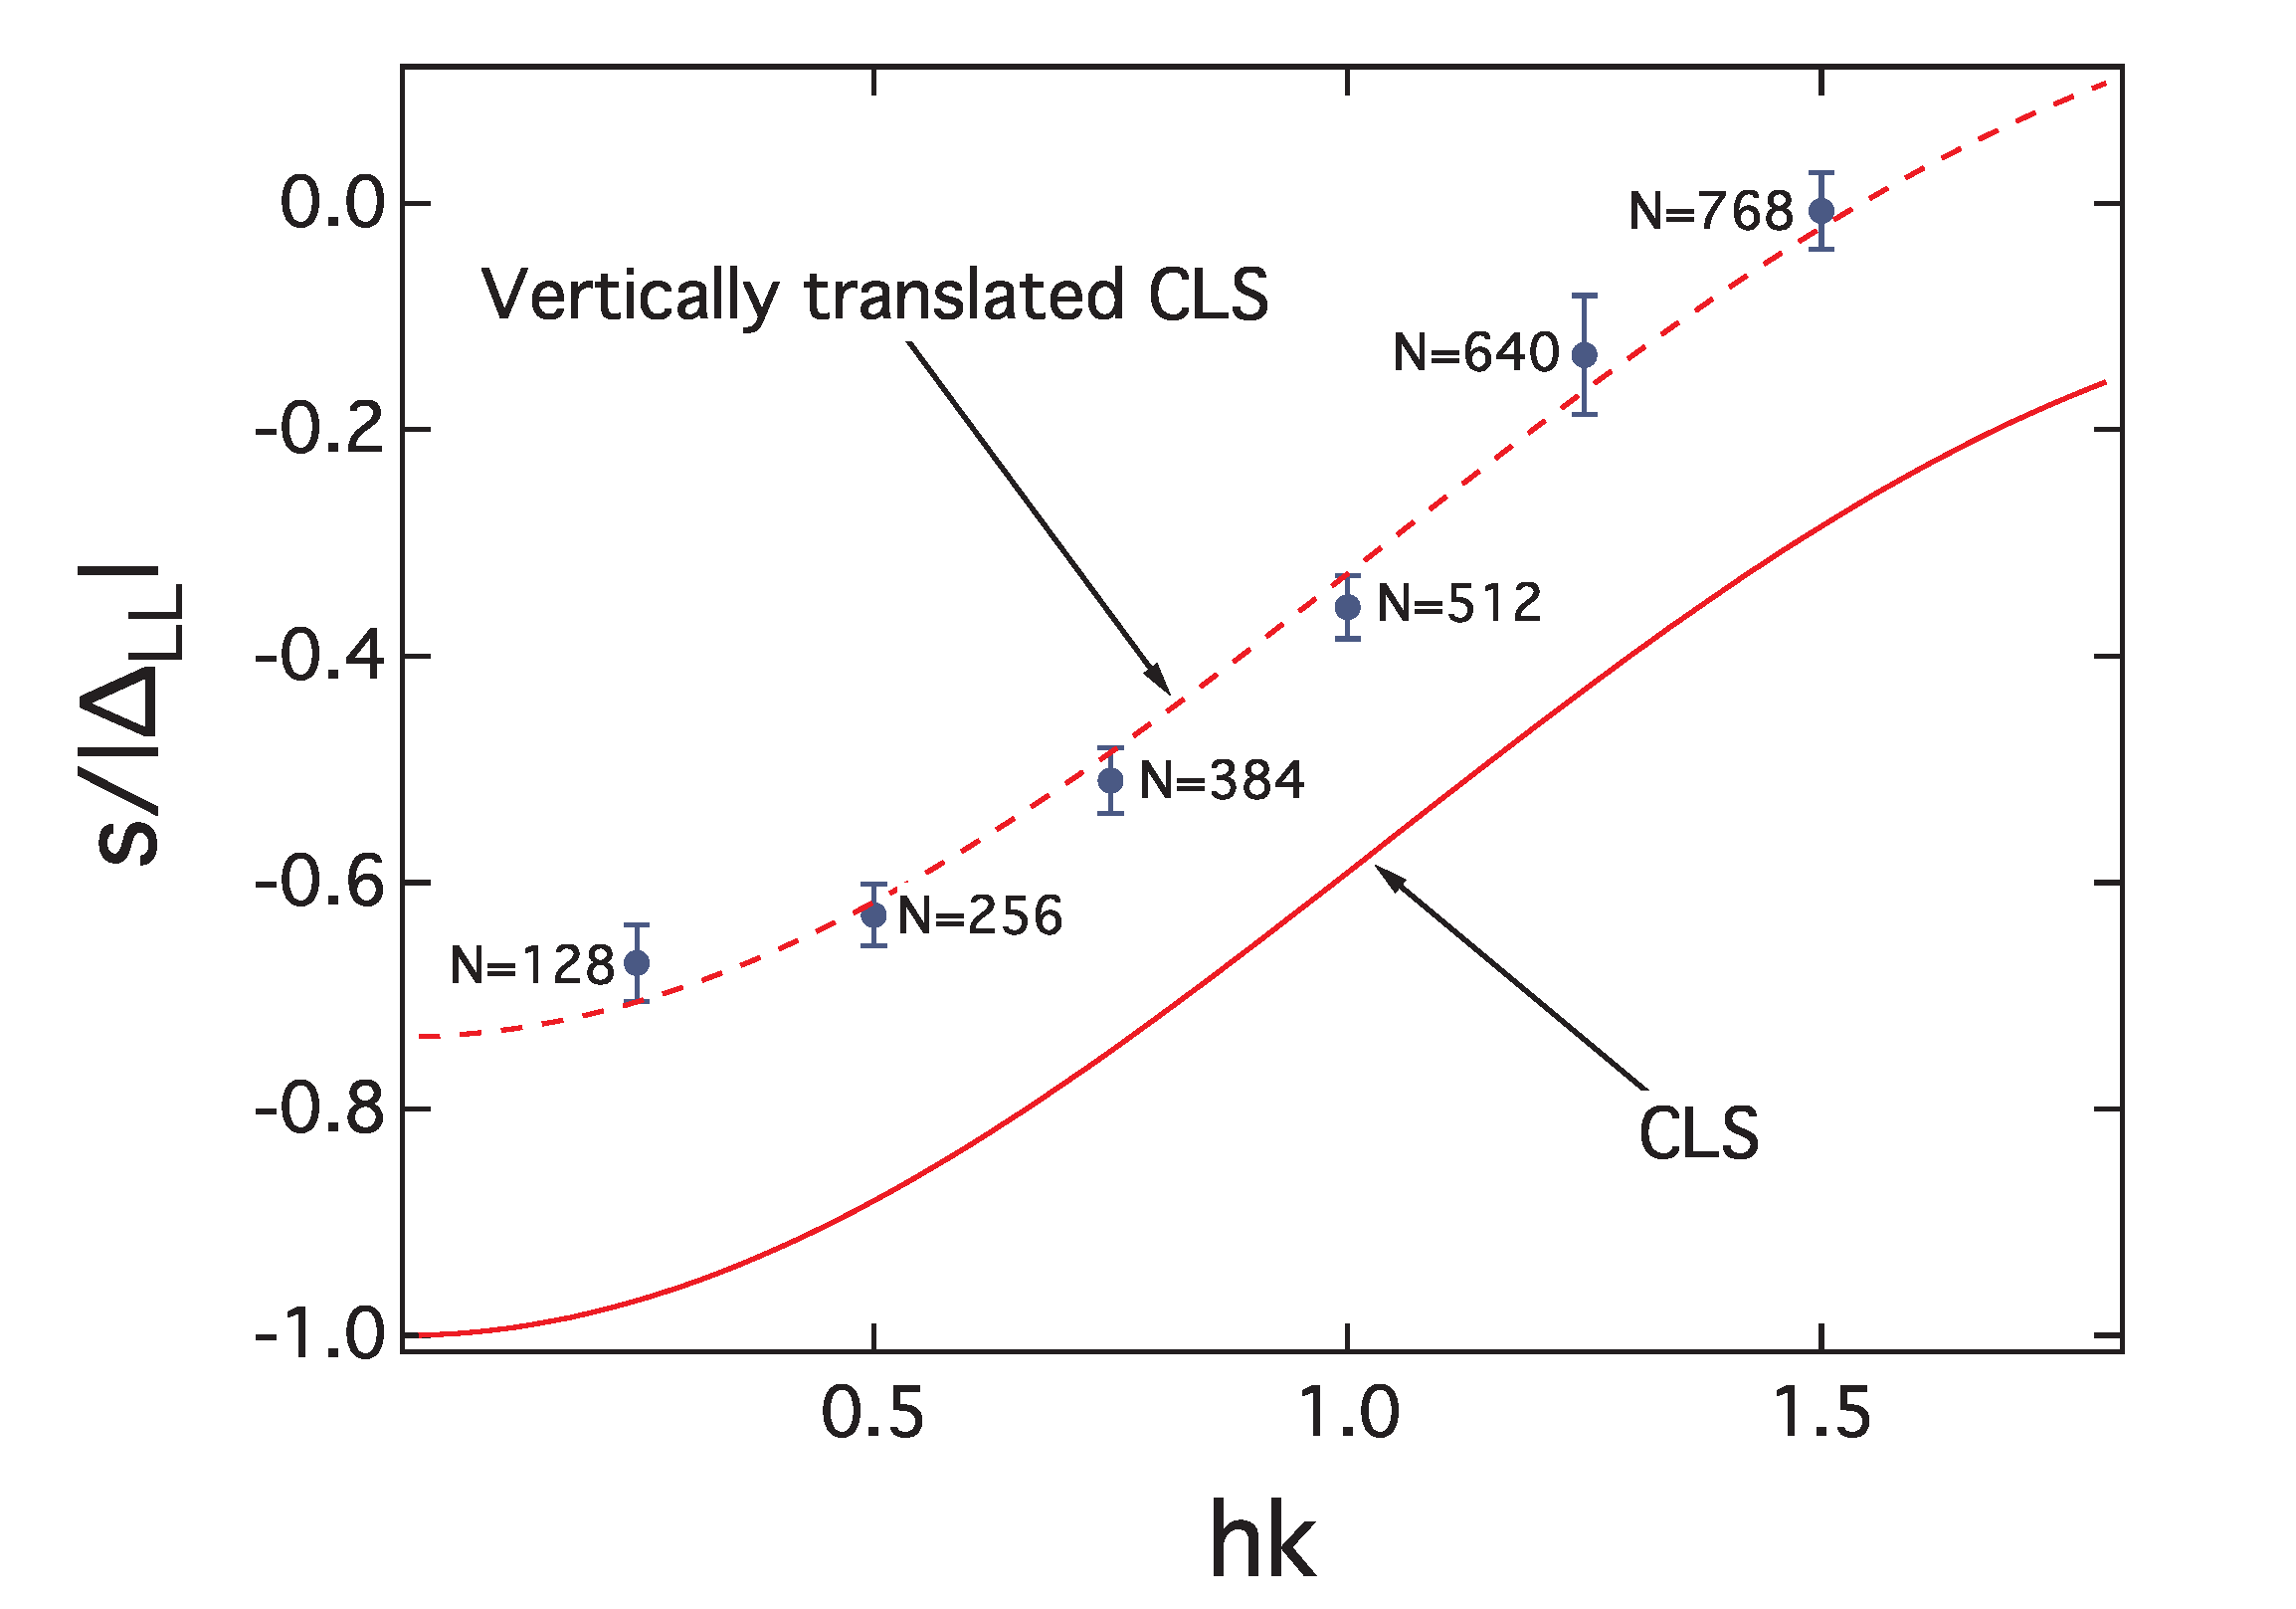
\includegraphics[width=\textwidth]{CLS.pdf}
\end{center}
\caption{The shift of the absorption line $s$ versus the thickness $h$ in a dense gas of moving atoms. $\Delta_{LL}$ is the standard LL shift. The shift is defined as [[SHIFT OF MAXIMUM, SHIFT OF FITTED LORENTZIAN, SHIFT OF ...]].  The fixed parameters are $\rho=2$, $A=256$, and [[$u=???$]]. [[REMOVE k, SPECIAL UNITS]]}
\label{CLS}
\end{figure}

\subsection{Broadening of the Dicke-narrowed lineshape in a dense gas}

By varying the density of the gas, we found new signs of cooperative effects in the absorption spectra.

\begin{figure}[h!]
\begin{center}
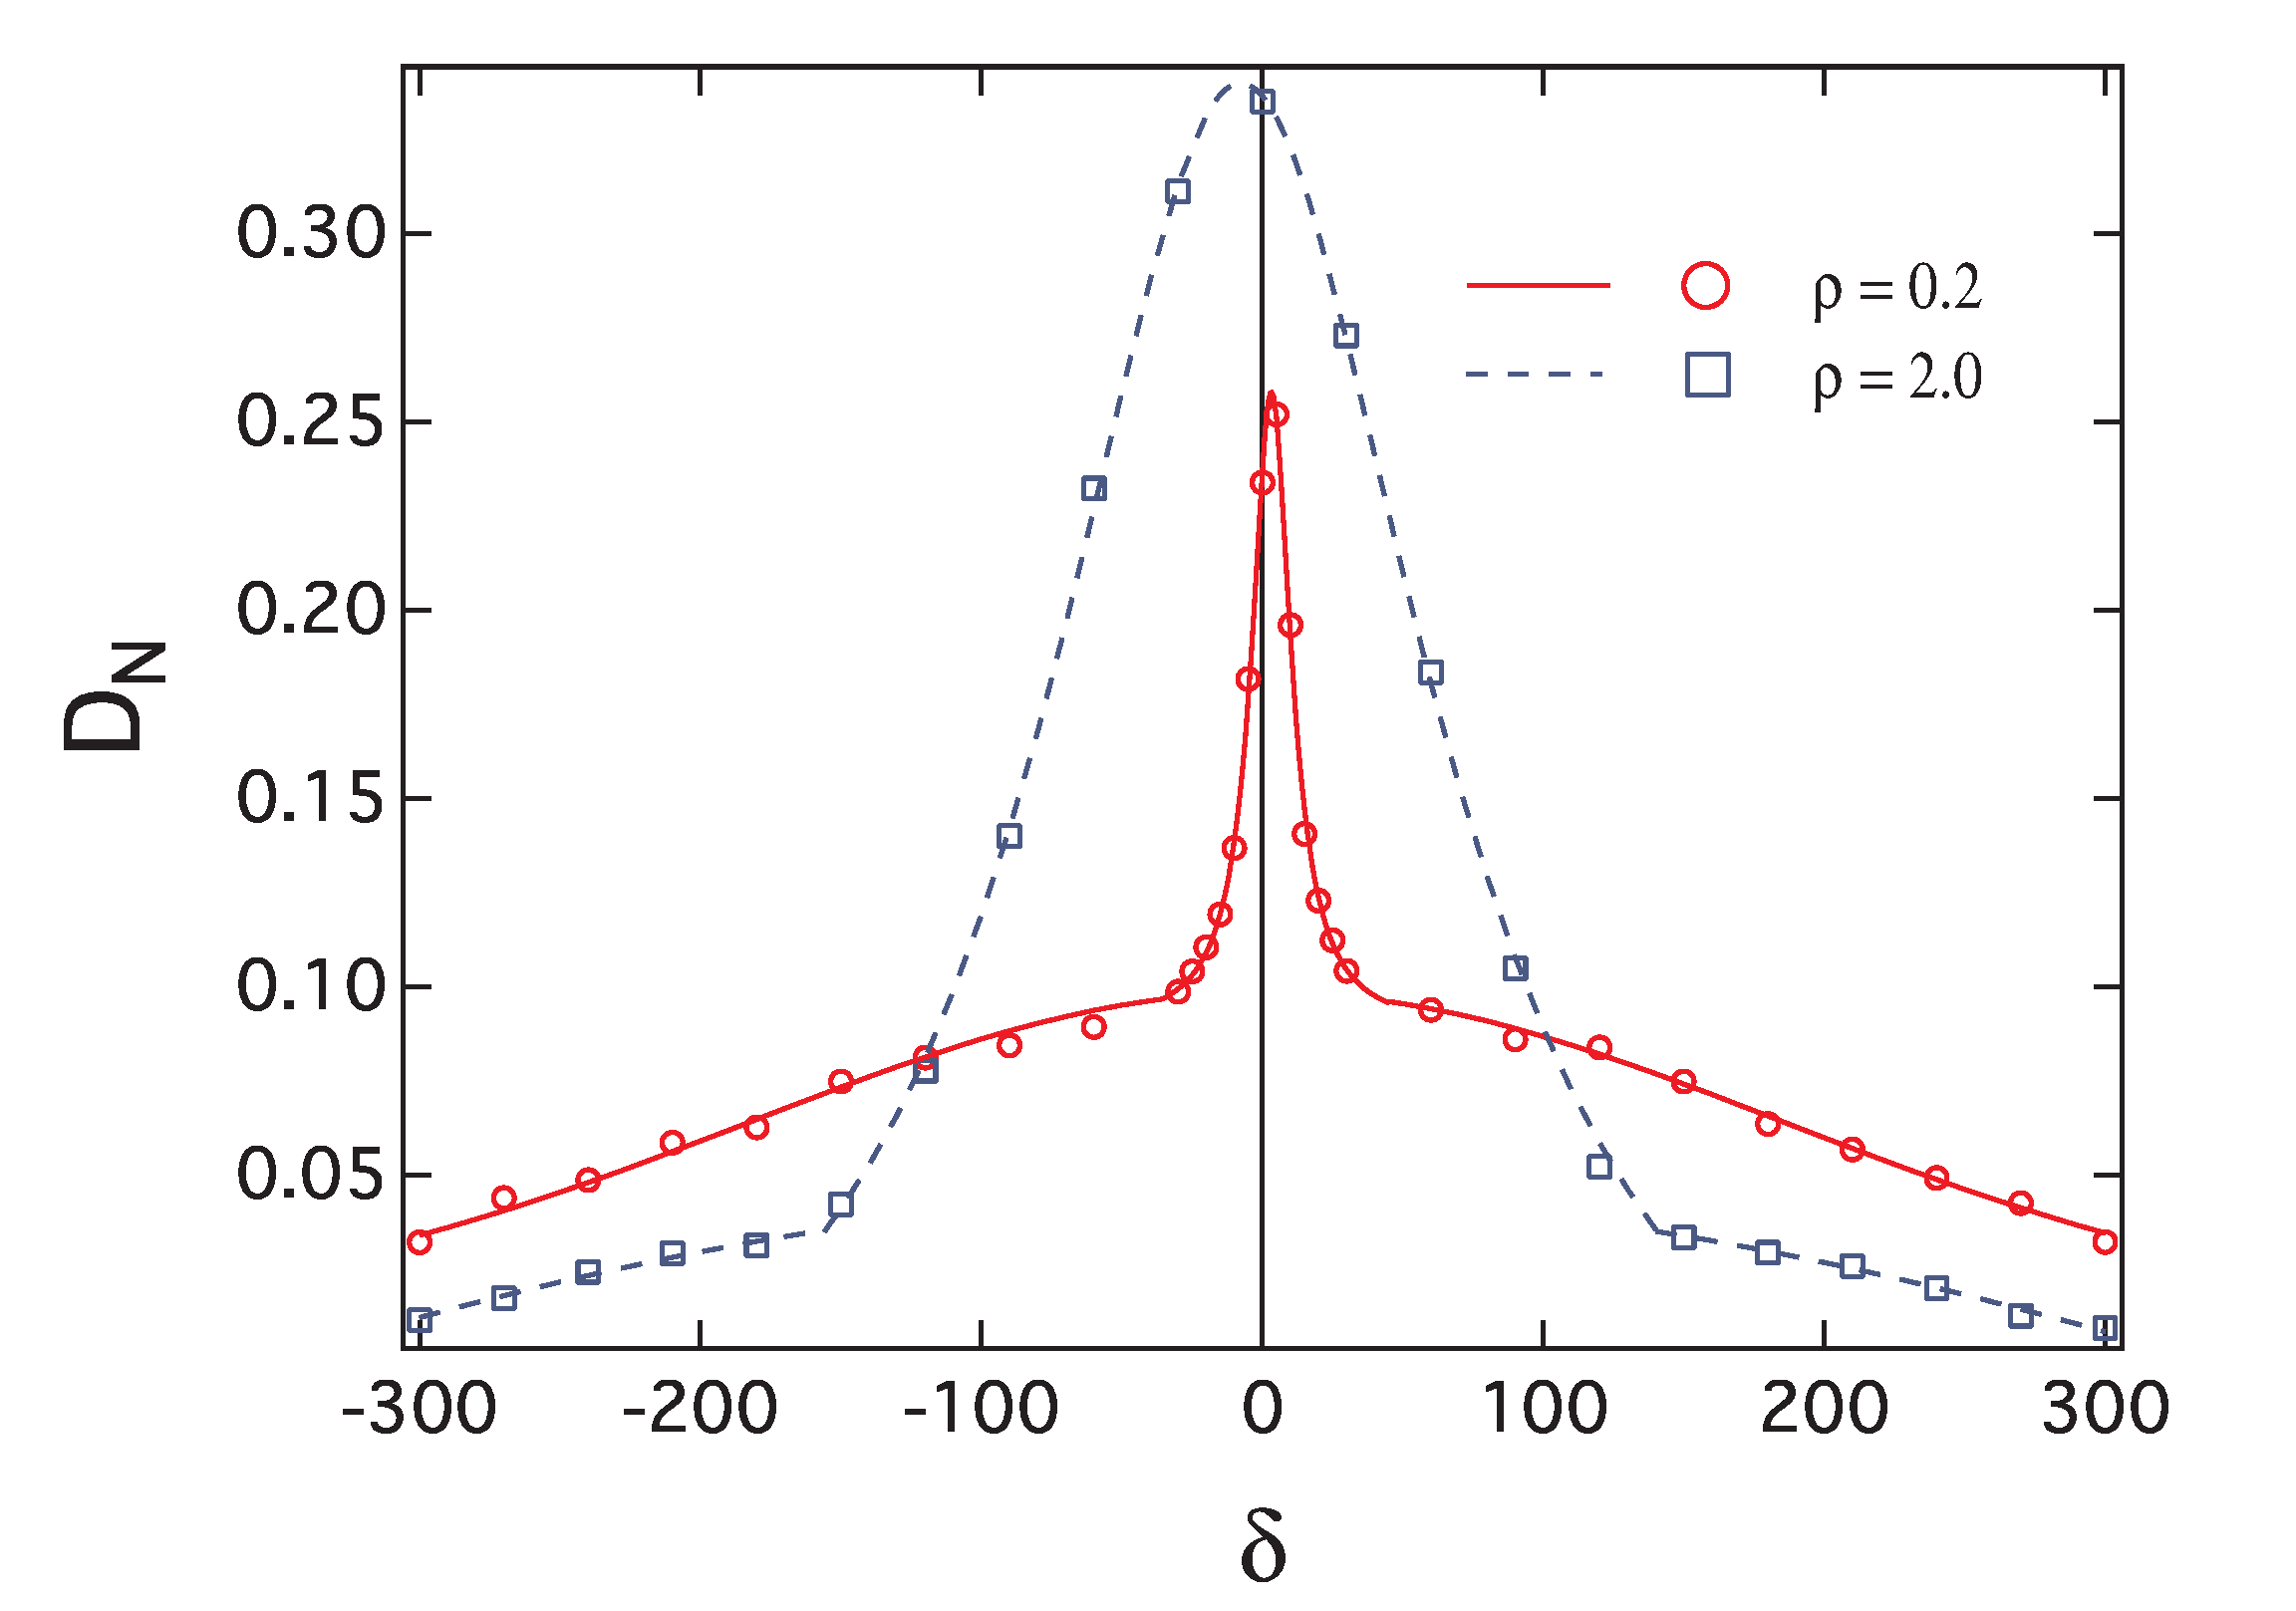
\includegraphics[width=\textwidth]{DICKE.pdf}
\end{center}
\caption{Optical thickness $D_N$ versus detuning $\delta$ in two samples with different densities but the same number of atoms $N=256$. The thickness of the disk is $h=5$ (red circles) and $0.5$ (blue boxes), respectively. [[THE LINES ARE DRAWN TO GUIDE THE EYE?]]. In both cases the rms velocity of the atoms is [[IMPOSSIBLE $u=5$]], and the radius of the disk is the usual $R=\sqrt{256/\pi}$. The collision radius of an atom is $r_a=0.01$, so atom-atom collisions are very rare.}
\label{DICKE}
\end{figure}

As shown in Fig.~\ref{DICKE},  in a dilute gas ($\rho =0.2$), a sharp Lorentzian peak arises near resonance over the base of  a Gaussian profile due to inhomogeneous broadening. This is typical of Dicke narrowing. Note that in Sec.~\ref{SMAG} we also have a narrowing effect on the lineshape from collisions, but what we observed there is more like a continuous transition from a Gaussian to a Lorentzian, not an abrupt Lorentzian peak over a Gaussian base. We surmise that here the appearance of a Dicke narrowed spectrum does not result solely from collisions; in order to produce the final lineshape, dipole-dipole interactions (i.e. cooperative effects) must also be present.

In the high density regime ($\rho =2$), the spectrum is still composed of two parts: Gaussian in the side wings and Lorentzian at the center. However, the central peak, presumable a vestige of Dicke narrowing, is remarkably broadened even though the collision rate is much higher than for the density $\rho =0.2$.

\begin{figure}[h!]
\begin{center}
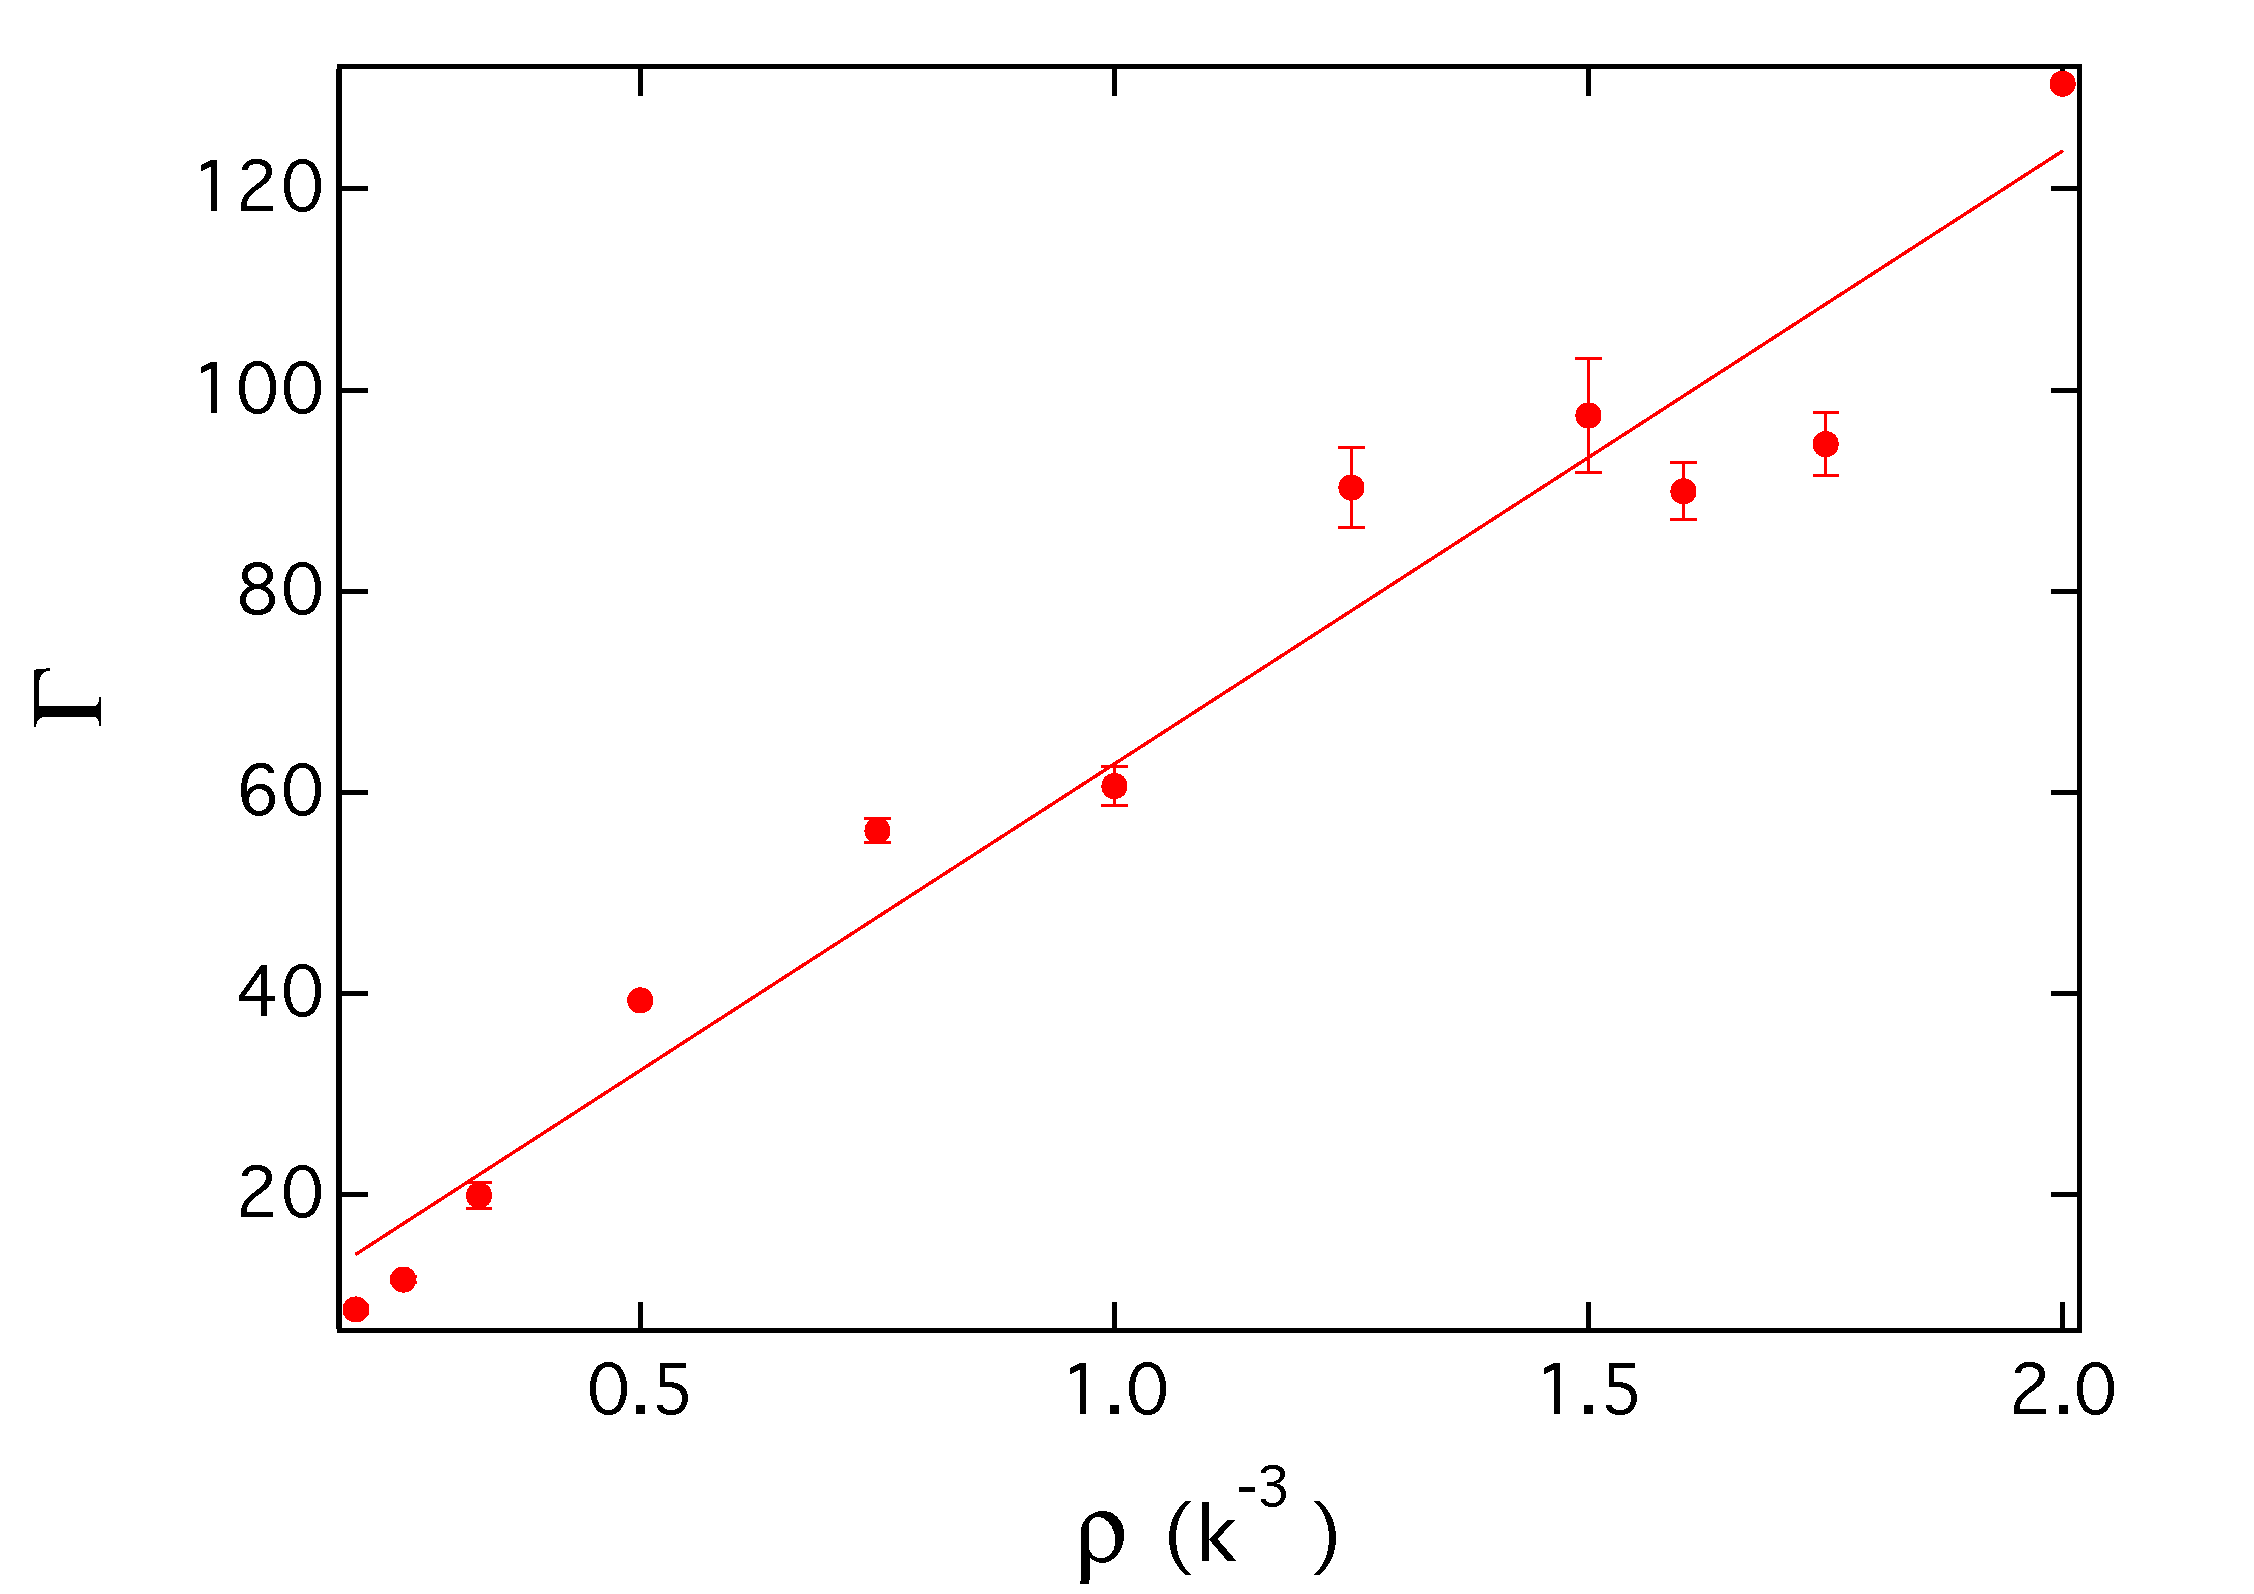
\includegraphics[width=\textwidth]{FWHM.pdf}
\end{center}
\caption{FWHM of the Lorentzian peak [[CALL IT SOMETHING, SAY $\Gamma$]] vs.\ density [[say, $\rho$]] for the fixed number of atoms $N=256$. The density is changed by varying the thickness of the disk with the usual area $A=256$. [[As before, the motional broadening is specified by $u=xxx$]]. [[The collision radius is xxxx, so atom-atom collisions are rare]].}
\label{FWHM}
\end{figure}

Let us finally consider Fig.~\ref{FWHM} that presents the width of the central peak as a function of the density of the gas. [[HOW IS THE WIDTH OBTAINED? LORENTZIAN WIDTH? LITERALLY, FWHM?]]
Recall the results we obtained in Sec.~\ref{SMAG}, without the dipole-dipole interactions, that a higher frequency of either atom-wall collisions or atom-atom collisions would narrow the lineshape. As increasing density in Fig.~\ref{FWHM} implies an increasing collision rate, the behavior of the linewidth is opposite to what one would expect for Dicke narrowing. Evidently, the width of the center peak of the spectrum keeps increasing because of the dipole-dipole interactions as the density goes up.  We surmise that this broadening is a cooperative effect due to rescattering of light between the atoms.
